\documentclass[3p,a4paper,11pt,review]{elsarticle}

\usepackage{lineno}
\usepackage{hyperref}
\usepackage{latexsym}
\usepackage{color}
\usepackage[table]{xcolor}
\usepackage{mathrsfs}
\usepackage{amssymb,amstext,amsfonts,amsmath,amsthm}
\usepackage{bm}
\usepackage{subcaption}
\usepackage[utf8]{inputenc} 
\usepackage[english]{babel}
\usepackage{hyphenat}
\usepackage{calc}
\usepackage{graphicx,import}

\usepackage{soul}

\usepackage{caption}
\usepackage{subcaption}

\usepackage{arydshln}
\usepackage{natbib}
\usepackage[misc,geometry]{ifsym} 
\usepackage{empheq}
\usepackage{longtable}
\usepackage{comment}

\bibliographystyle{plain}\biboptions{authoryear}


\usepackage{lineno}
\newcommand*\patchAmsMathEnvironmentForLineno[1]{%
	\expandafter\let\csname old#1\expandafter\endcsname\csname #1\endcsname
	\expandafter\let\csname oldend#1\expandafter\endcsname\csname end#1\endcsname
	\renewenvironment{#1}%
	{\linenomath\csname old#1\endcsname}%
	{\csname oldend#1\endcsname\endlinenomath}}%
\newcommand*\patchBothAmsMathEnvironmentsForLineno[1]{%
	\patchAmsMathEnvironmentForLineno{#1}%
	\patchAmsMathEnvironmentForLineno{#1*}}%
\AtBeginDocument{%
	\patchBothAmsMathEnvironmentsForLineno{equation}%
	\patchBothAmsMathEnvironmentsForLineno{align}%
	\patchBothAmsMathEnvironmentsForLineno{flalign}%
	\patchBothAmsMathEnvironmentsForLineno{alignat}%
	\patchBothAmsMathEnvironmentsForLineno{gather}%
	\patchBothAmsMathEnvironmentsForLineno{multline}%
}

\usepackage[]{algorithm2e}

\hyphenation{ONSAS}

\usepackage{tikz}
\usetikzlibrary{shapes,arrows}

\usepackage{relsize}

\definecolor{darkcandyapplered}{rgb}{0.64, 0.0, 0.0}
\definecolor{darkred}{rgb}{0.55, 0.0, 0.0}


\usepackage{bbm}



\usepackage{enumitem,amssymb}
\newlist{todolist}{itemize}{2}
\setlist[todolist]{label=$\square$}
%
\usepackage{pifont}
%
\newcommand{\failed}{%
	\rlap{\raisebox{0.3ex}{\hspace{0.4ex}\scriptsize \ding{56}}}$\square$%
}
%
\newcommand{\done}{%
	\rlap{\raisebox{0.3ex}{\hspace{0.4ex}\tiny \ding{52}}}$\square$%
}

\newcommand{\miparra}[1]{\vspace{5mm} \textbf{#1}\\}

\journal{?}

\begin{document}
	
	
	\begin{frontmatter}
		
		\title{A Consistent Co-rotational Formulation for Quasi-Steady Aerodynamic Nonlinear Analysis of Frame Structures}
		
		\author[1]{Mauricio C. Vanzulli}
		\author[2]{Jorge M. Pérez Zerpa}
		
		\address[1]{Instituto de Ingeniería Mecánica y Producción Industrial, Facultad de Ingeniería, Universidad de la República, Montevideo, Uruguay}
		
		% Corresponding author
		\address[2]{Instituto de Estructuras y Transporte, Facultad de Ingeniería, Universidad de la República, Montevideo, Uruguay}  
		
	\end{frontmatter}


\section{Numerical results}


\subsection{Example 1}

\newcommand{\CircularReconfigurationL}{1}
\newcommand{\CircularReconfigurationd}{1}
\newcommand{\CircularReconfigurationE}{30}
\newcommand{\CircularReconfigurationrho}{7000}
\newcommand{\CircularReconfigurationrhoFluid}{1020}
\newcommand{\CircularReconfigurationcd}{1.2}
\newcommand{\CircularReconfigurationcycdCaseOne}{1.6681}
\newcommand{\CircularReconfigurationcycdCaseTwo}{4.6416}
\newcommand{\CircularReconfigurationfulidVelCaseOne}{6.3355}
\newcommand{\CircularReconfigurationfulidVelCaseTwo}{1.0568}
\newcommand{\CircularReconfigurationtolF}{1}
\newcommand{\CircularReconfigurationtolU}{1}
\newcommand{\CircularReconfigurationdeltaT}{0.05}
\newcommand{\CircularReconfigurationfinalTime}{7}
\newcommand{\CircularReconfigurationtc}{7}
\newcommand{\CircularReconfigurationvaOne}{0.005}
\newcommand{\CircularReconfigurationvaTwo}{0.012}
\newcommand{\CircularReconfigurationvaThree}{0.029}
\newcommand{\CircularReconfigurationvaFour}{0.072}
\newcommand{\CircularReconfigurationvaFive}{0.176}
\newcommand{\CircularReconfigurationvaSix}{0.432}
\newcommand{\CircularReconfigurationvaSeven}{1.057}
\newcommand{\CircularReconfigurationvaEight}{2.588}
\newcommand{\CircularReconfigurationvaNine}{6.336}
\newcommand{\CircularReconfigurationvaTen}{15.512}
\newcommand{\CircularReconfigurationexecTimeRatio}{    6}


The parameters of this example are:

\begin{itemize}
	\item $d= \CircularReconfigurationd$ m.
	\item $L = \CircularReconfigurationL$ m.
	\item $v_a \in \{ \CircularReconfigurationvaOne, \CircularReconfigurationvaTwo, \CircularReconfigurationvaThree, \CircularReconfigurationvaFour, \CircularReconfigurationvaFive, \CircularReconfigurationvaSix, \CircularReconfigurationvaSeven, \CircularReconfigurationvaEight, \CircularReconfigurationvaNine, \CircularReconfigurationvaTen \}$ all in m/s.
	\item $\rho_f = \CircularReconfigurationrhoFluid$ kg/m$^3$.
	\item $E = \CircularReconfigurationE$ MPa and density $\rho = \CircularReconfigurationrho$ kg/m$^3$.
	\item $tol_r = \CircularReconfigurationtolF\times 10^{-7}$.
	\item $tol_u = \CircularReconfigurationtolU0^{-15}$.
%	\item $\alpha = \CircularReconfigurationalphaEnd^{\circ}$
\end{itemize}

\subsubsection{Example 1: Numerical results}

\begin{itemize}
	\item F1 and F2 works for static case with $v_a \leq \CircularReconfigurationvaFour$ m/s. 

	\item It is reported that, for $v_a = \CircularReconfigurationvaFour$ m/s and using 20 elements, the formulation F3 requires $\CircularReconfigurationexecTimeRatio$ times the execution time required by F1 or F2 formulations.
\end{itemize}



\begin{figure}[htb]
	\begin{subfigure}{.5\textwidth}
		\centering
		\resizebox{.93\textwidth}{!}{% Title: Figure 1
% Creator: GL2PS 1.4.2, (C) 1999-2020 C. Geuzaine
% For: Octave
% CreationDate: Mon Jan 23 17:15:09 2023
\setlength{\unitlength}{1pt}
\begin{picture}(0,0)
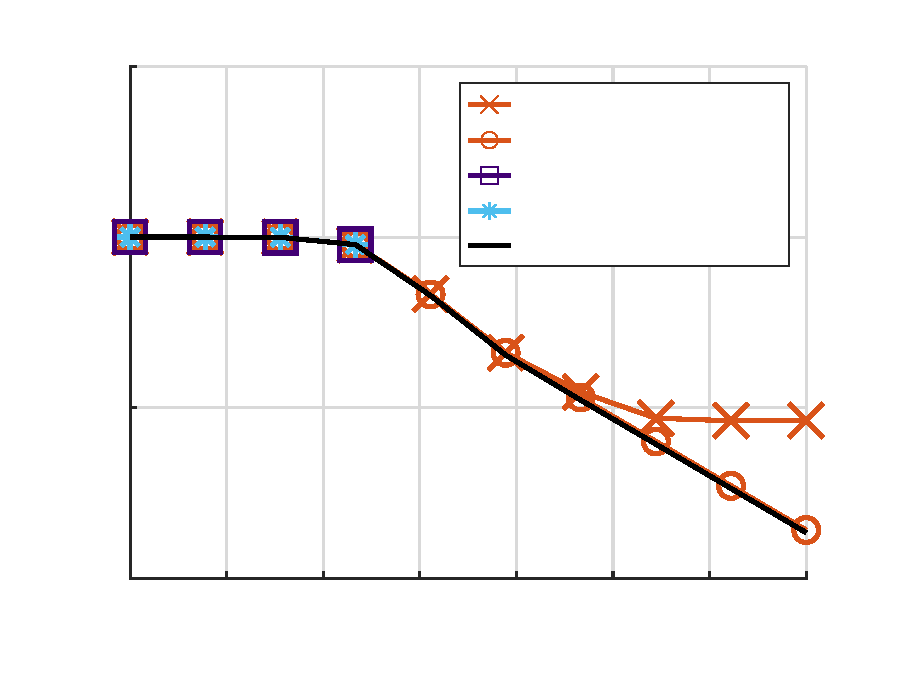
\includegraphics[scale=1]{ex1CyR-inc}
\end{picture}%
\begin{picture}(418,314)(0,0)
\fontsize{14}{0}\selectfont\put(54.4343,33.9551){\makebox(0,0)[t]{\textcolor[rgb]{0.15,0.15,0.15}{{$10^{-2}$}}}}
\fontsize{14}{0}\selectfont\put(100.793,33.9551){\makebox(0,0)[t]{\textcolor[rgb]{0.15,0.15,0.15}{{$10^{-1}$}}}}
\fontsize{14}{0}\selectfont\put(147.152,33.9551){\makebox(0,0)[t]{\textcolor[rgb]{0.15,0.15,0.15}{{$10^{0}$}}}}
\fontsize{14}{0}\selectfont\put(193.511,33.9551){\makebox(0,0)[t]{\textcolor[rgb]{0.15,0.15,0.15}{{$10^{1}$}}}}
\fontsize{14}{0}\selectfont\put(239.87,33.9551){\makebox(0,0)[t]{\textcolor[rgb]{0.15,0.15,0.15}{{$10^{2}$}}}}
\fontsize{14}{0}\selectfont\put(286.229,33.9551){\makebox(0,0)[t]{\textcolor[rgb]{0.15,0.15,0.15}{{$10^{3}$}}}}
\fontsize{14}{0}\selectfont\put(332.588,33.9551){\makebox(0,0)[t]{\textcolor[rgb]{0.15,0.15,0.15}{{$10^{4}$}}}}
\fontsize{14}{0}\selectfont\put(378.946,33.9551){\makebox(0,0)[t]{\textcolor[rgb]{0.15,0.15,0.15}{{$10^{5}$}}}}
\fontsize{14}{0}\selectfont\put(47.4448,44.4548){\makebox(0,0)[r]{\textcolor[rgb]{0.15,0.15,0.15}{{$10^{-2}$}}}}
\fontsize{14}{0}\selectfont\put(47.4448,126.452){\makebox(0,0)[r]{\textcolor[rgb]{0.15,0.15,0.15}{{$10^{-1}$}}}}
\fontsize{14}{0}\selectfont\put(47.4448,208.449){\makebox(0,0)[r]{\textcolor[rgb]{0.15,0.15,0.15}{{$10^{0}$}}}}
\fontsize{14}{0}\selectfont\put(47.4448,290.447){\makebox(0,0)[r]{\textcolor[rgb]{0.15,0.15,0.15}{{$10^{1}$}}}}
\fontsize{15}{0}\selectfont\put(216.69,16.9551){\makebox(0,0)[t]{\textcolor[rgb]{0.15,0.15,0.15}{{ $c_yc_d$ }}}}
\fontsize{15}{0}\selectfont\put(15.4448,167.451){\rotatebox{90}{\makebox(0,0)[b]{\textcolor[rgb]{0.15,0.15,0.15}{{$R$}}}}}
\fontsize{12}{0}\selectfont\put(240.952,271.952){\makebox(0,0)[l]{\textcolor[rgb]{0,0,0}{{F3 (2 elements)}}}}
\fontsize{12}{0}\selectfont\put(240.952,254.954){\makebox(0,0)[l]{\textcolor[rgb]{0,0,0}{{F3 (20 elements)}}}}
\fontsize{12}{0}\selectfont\put(240.952,237.955){\makebox(0,0)[l]{\textcolor[rgb]{0,0,0}{{F1 or F2 (2 elements)}}}}
\fontsize{12}{0}\selectfont\put(240.952,220.957){\makebox(0,0)[l]{\textcolor[rgb]{0,0,0}{{F1 or F2 (20 elements)}}}}
\fontsize{12}{0}\selectfont\put(240.952,204.459){\makebox(0,0)[l]{\textcolor[rgb]{0,0,0}{{Reference solution}}}}
\end{picture}
}
		\caption{Scaled Cauchy $c_yc_d$ number vs reconfiguration number $\mathcal{R}$.}
		\label{fig:ex1CuachyVsR}
	\end{subfigure}
	\begin{subfigure}{0.5\textwidth}
		\centering
		\resizebox{.95\textwidth}{!}{% Title: Figure 2
% Creator: GL2PS 1.4.2, (C) 1999-2020 C. Geuzaine
% For: Octave
% CreationDate: Mon Jan 23 17:16:57 2023
\setlength{\unitlength}{1pt}
\begin{picture}(0,0)
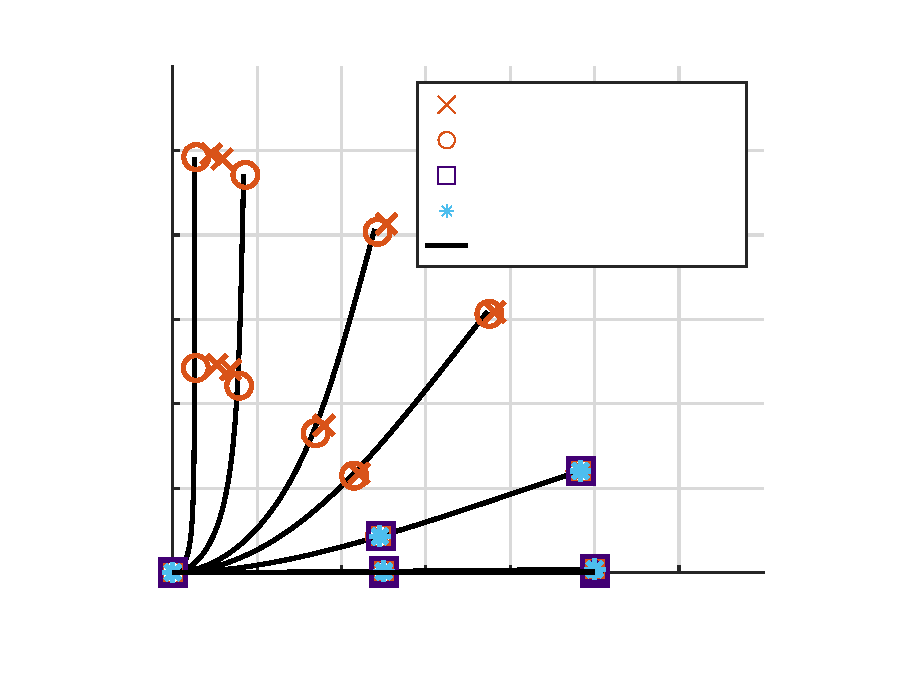
\includegraphics[scale=1]{ex1deformed-inc}
\end{picture}%
\begin{picture}(418,314)(0,0)
\fontsize{14}{0}\selectfont\put(74.9453,36.9556){\makebox(0,0)[t]{\textcolor[rgb]{0.15,0.15,0.15}{{0}}}}
\fontsize{14}{0}\selectfont\put(115.444,36.9556){\makebox(0,0)[t]{\textcolor[rgb]{0.15,0.15,0.15}{{0.2}}}}
\fontsize{14}{0}\selectfont\put(155.942,36.9556){\makebox(0,0)[t]{\textcolor[rgb]{0.15,0.15,0.15}{{0.4}}}}
\fontsize{14}{0}\selectfont\put(196.441,36.9556){\makebox(0,0)[t]{\textcolor[rgb]{0.15,0.15,0.15}{{0.6}}}}
\fontsize{14}{0}\selectfont\put(236.94,36.9556){\makebox(0,0)[t]{\textcolor[rgb]{0.15,0.15,0.15}{{0.8}}}}
\fontsize{14}{0}\selectfont\put(277.438,36.9556){\makebox(0,0)[t]{\textcolor[rgb]{0.15,0.15,0.15}{{1}}}}
\fontsize{14}{0}\selectfont\put(317.937,36.9556){\makebox(0,0)[t]{\textcolor[rgb]{0.15,0.15,0.15}{{1.2}}}}
\fontsize{14}{0}\selectfont\put(67.9332,47.4552){\makebox(0,0)[r]{\textcolor[rgb]{0.15,0.15,0.15}{{0}}}}
\fontsize{14}{0}\selectfont\put(67.9332,87.9538){\makebox(0,0)[r]{\textcolor[rgb]{0.15,0.15,0.15}{{0.2}}}}
\fontsize{14}{0}\selectfont\put(67.9332,128.452){\makebox(0,0)[r]{\textcolor[rgb]{0.15,0.15,0.15}{{0.4}}}}
\fontsize{14}{0}\selectfont\put(67.9332,168.951){\makebox(0,0)[r]{\textcolor[rgb]{0.15,0.15,0.15}{{0.6}}}}
\fontsize{14}{0}\selectfont\put(67.9332,209.45){\makebox(0,0)[r]{\textcolor[rgb]{0.15,0.15,0.15}{{0.8}}}}
\fontsize{14}{0}\selectfont\put(67.9332,249.948){\makebox(0,0)[r]{\textcolor[rgb]{0.15,0.15,0.15}{{1}}}}
\fontsize{20}{0}\selectfont\put(216.69,21.9556){\makebox(0,0)[t]{\textcolor[rgb]{0.15,0.15,0.15}{{ $x$ [m] }}}}
\fontsize{20}{0}\selectfont\put(44.9332,168.951){\rotatebox{90}{\makebox(0,0)[b]{\textcolor[rgb]{0.15,0.15,0.15}{{$y$ [m]}}}}}
\fontsize{12}{0}\selectfont\put(220.441,271.952){\makebox(0,0)[l]{\textcolor[rgb]{0,0,0}{{F3 (2 elements)}}}}
\fontsize{12}{0}\selectfont\put(220.441,254.954){\makebox(0,0)[l]{\textcolor[rgb]{0,0,0}{{F3 (20 elements)}}}}
\fontsize{12}{0}\selectfont\put(220.441,237.955){\makebox(0,0)[l]{\textcolor[rgb]{0,0,0}{{F1 or F2 (2 elements)}}}}
\fontsize{12}{0}\selectfont\put(220.441,220.957){\makebox(0,0)[l]{\textcolor[rgb]{0,0,0}{{F1 or F2 (20 elements)}}}}
\fontsize{12}{0}\selectfont\put(220.441,204.459){\makebox(0,0)[l]{\textcolor[rgb]{0,0,0}{{Reference solution}}}}
\end{picture}
}
		\caption{Deformed configurations for different $c_yc_d$ numbers.}
		\label{fig:ex1DeformedConfig}
	\end{subfigure}
	\caption{Example 1: Drag reconfiguration validation against (Gosselin et Al, 2010).}
	\label{fig:ex1StaticRecValidation}
\end{figure}



\begin{figure}[htb]
	\begin{subfigure}{.5\textwidth}
		\centering
		\resizebox{.93\textwidth}{!}{\input{ex1UyAvsTimeWindVelCase1.tex}}
		\caption{$u_y(t)$ for $c_yc_d = \CircularReconfigurationcycdCaseOne \times 10^4$ (Case 1).}
		\label{fig:reconfigurationBeamCase1UyA}
	\end{subfigure}
	\begin{subfigure}{0.5\textwidth}
		\centering
		\resizebox{.95\textwidth}{!}{% Title: Figure 7
% Creator: GL2PS 1.4.2, (C) 1999-2020 C. Geuzaine
% For: Octave
% CreationDate: Mon Jan 23 17:17:30 2023
\setlength{\unitlength}{1pt}
\begin{picture}(0,0)
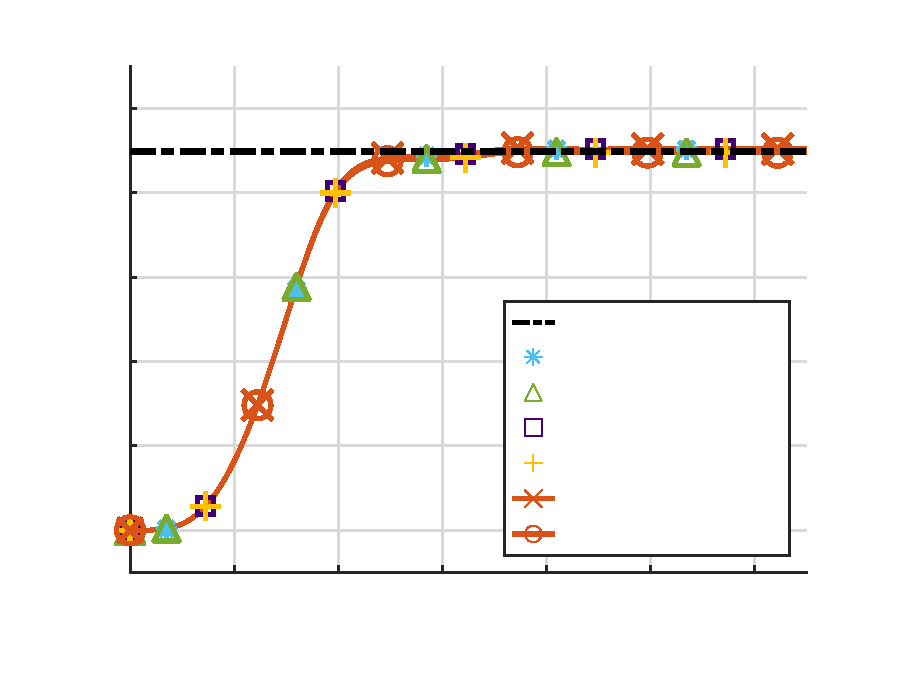
\includegraphics[scale=1]{ex1UyAvsTimeWindVelCase2-inc}
\end{picture}%
\begin{picture}(418,314)(0,0)
\fontsize{14}{0}\selectfont\put(54.4343,36.9563){\makebox(0,0)[t]{\textcolor[rgb]{0.15,0.15,0.15}{{0}}}}
\fontsize{14}{0}\selectfont\put(104.359,36.9563){\makebox(0,0)[t]{\textcolor[rgb]{0.15,0.15,0.15}{{2}}}}
\fontsize{14}{0}\selectfont\put(154.284,36.9563){\makebox(0,0)[t]{\textcolor[rgb]{0.15,0.15,0.15}{{4}}}}
\fontsize{14}{0}\selectfont\put(204.209,36.9563){\makebox(0,0)[t]{\textcolor[rgb]{0.15,0.15,0.15}{{6}}}}
\fontsize{14}{0}\selectfont\put(254.134,36.9563){\makebox(0,0)[t]{\textcolor[rgb]{0.15,0.15,0.15}{{8}}}}
\fontsize{14}{0}\selectfont\put(304.059,36.9563){\makebox(0,0)[t]{\textcolor[rgb]{0.15,0.15,0.15}{{10}}}}
\fontsize{14}{0}\selectfont\put(353.984,36.9563){\makebox(0,0)[t]{\textcolor[rgb]{0.15,0.15,0.15}{{12}}}}
\fontsize{14}{0}\selectfont\put(47.4448,67.7052){\makebox(0,0)[r]{\textcolor[rgb]{0.15,0.15,0.15}{{0}}}}
\fontsize{14}{0}\selectfont\put(47.4448,108.204){\makebox(0,0)[r]{\textcolor[rgb]{0.15,0.15,0.15}{{0.2}}}}
\fontsize{14}{0}\selectfont\put(47.4448,148.702){\makebox(0,0)[r]{\textcolor[rgb]{0.15,0.15,0.15}{{0.4}}}}
\fontsize{14}{0}\selectfont\put(47.4448,189.201){\makebox(0,0)[r]{\textcolor[rgb]{0.15,0.15,0.15}{{0.6}}}}
\fontsize{14}{0}\selectfont\put(47.4448,229.699){\makebox(0,0)[r]{\textcolor[rgb]{0.15,0.15,0.15}{{0.8}}}}
\fontsize{14}{0}\selectfont\put(47.4448,270.197){\makebox(0,0)[r]{\textcolor[rgb]{0.15,0.15,0.15}{{1}}}}
\fontsize{20}{0}\selectfont\put(216.69,21.9563){\makebox(0,0)[t]{\textcolor[rgb]{0.15,0.15,0.15}{{ $t$ [s] }}}}
\fontsize{20}{0}\selectfont\put(24.4448,168.951){\rotatebox{90}{\makebox(0,0)[b]{\textcolor[rgb]{0.15,0.15,0.15}{{$u_y$ node A [m]}}}}}
\fontsize{12}{0}\selectfont\put(261.952,167.44){\makebox(0,0)[l]{\textcolor[rgb]{0,0,0}{{Reference solution}}}}
\fontsize{12}{0}\selectfont\put(261.952,150.942){\makebox(0,0)[l]{\textcolor[rgb]{0,0,0}{{F1 (4 elements)}}}}
\fontsize{12}{0}\selectfont\put(261.952,133.944){\makebox(0,0)[l]{\textcolor[rgb]{0,0,0}{{F1 (20 elements)}}}}
\fontsize{12}{0}\selectfont\put(261.952,116.945){\makebox(0,0)[l]{\textcolor[rgb]{0,0,0}{{F2 (4 elements)}}}}
\fontsize{12}{0}\selectfont\put(261.952,99.9472){\makebox(0,0)[l]{\textcolor[rgb]{0,0,0}{{F2 (20 elements)}}}}
\fontsize{12}{0}\selectfont\put(261.952,82.9489){\makebox(0,0)[l]{\textcolor[rgb]{0,0,0}{{F3 (4 elements)}}}}
\fontsize{12}{0}\selectfont\put(261.952,65.9507){\makebox(0,0)[l]{\textcolor[rgb]{0,0,0}{{F3 (20 elements)}}}}
\end{picture}
}
		\caption{$u_y(t)$ for $c_yc_d = \CircularReconfigurationcycdCaseTwo \times 10^2$ (Case 2).}
		\label{fig:reconfigurationBeamCase2UyA}
	\end{subfigure}
	\caption{Example 1: Evolution of $u_y$ displacement of node A.}
	\label{fig:reconfigurationCantBeamDynamic}
\end{figure}

\clearpage

\subsection{Example 2}

\newcommand{\SimplePropellerL}{3}
\newcommand{\SimplePropellerd}{0.1}
\newcommand{\SimplePropellerEf}{2.1}
\newcommand{\SimplePropellerva}{1}
\newcommand{\SimplePropellerEr}{210}
\newcommand{\SimplePropellerrho}{6000}
\newcommand{\SimplePropellertolF}{1}
\newcommand{\SimplePropellertolU}{1}
\newcommand{\SimplePropellerdeltaT}{1}
\newcommand{\SimplePropellerfinalTime}{450}


The parameters of this example are:

\begin{itemize}
	\item $d= \SimplePropellerd$ m.
	\item $L = \SimplePropellerL $ m.
	\item $E_{flex} = \SimplePropellerEf$ kPa
	\item $E_{rigid} = \SimplePropellerEr$ GPa
	\item $\rho = \SimplePropellerrho$ kg/m$^3$
	\item $c_l = 0.2$
	\item $v_{a} = \SimplePropellerva$ m/s
	\item $tol_r = \SimplePropellertolF0^{-6}$
	\item $tol_u = \SimplePropellertolU0^{-12}$.
	\item $\Delta t = \SimplePropellerdeltaT$ s. 

\end{itemize}

\subsubsection{Example 2: Numerical results}

\begin{figure}[htb]
	\centering
	\resizebox{.5\textwidth}{!}{% Title: Figure 1
% Creator: GL2PS 1.4.2, (C) 1999-2020 C. Geuzaine
% For: Octave
% CreationDate: Tue Jan 24 13:40:19 2023
\setlength{\unitlength}{1pt}
\begin{picture}(0,0)
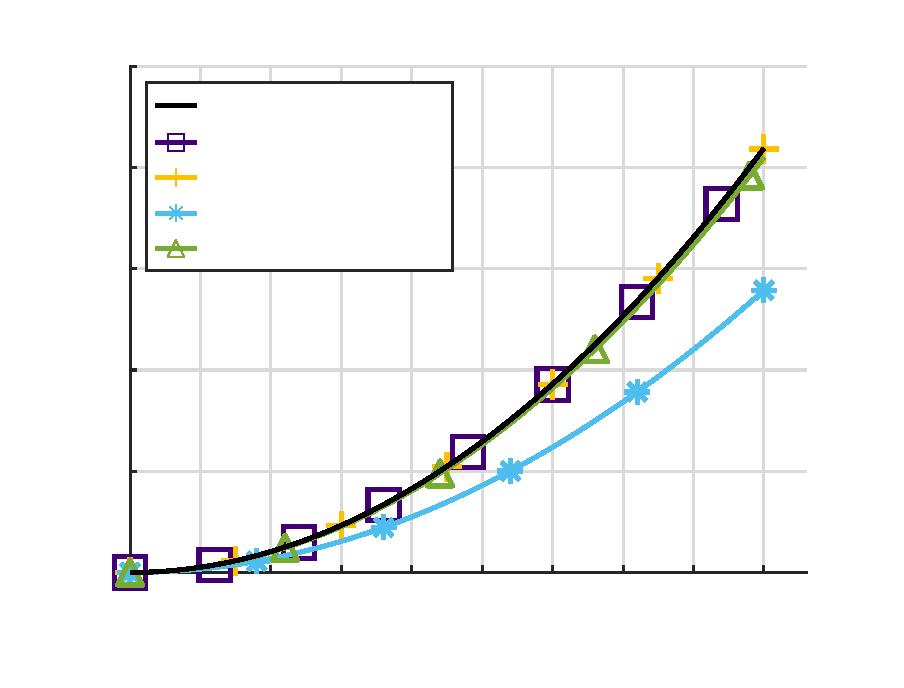
\includegraphics[scale=1]{valPropRigidThetaXO-inc}
\end{picture}%
\begin{picture}(418,314)(0,0)
\fontsize{14}{0}\selectfont\put(54.4343,36.9563){\makebox(0,0)[t]{\textcolor[rgb]{0.15,0.15,0.15}{{0}}}}
\fontsize{14}{0}\selectfont\put(88.2376,36.9563){\makebox(0,0)[t]{\textcolor[rgb]{0.15,0.15,0.15}{{50}}}}
\fontsize{14}{0}\selectfont\put(122.041,36.9563){\makebox(0,0)[t]{\textcolor[rgb]{0.15,0.15,0.15}{{100}}}}
\fontsize{14}{0}\selectfont\put(155.844,36.9563){\makebox(0,0)[t]{\textcolor[rgb]{0.15,0.15,0.15}{{150}}}}
\fontsize{14}{0}\selectfont\put(189.648,36.9563){\makebox(0,0)[t]{\textcolor[rgb]{0.15,0.15,0.15}{{200}}}}
\fontsize{14}{0}\selectfont\put(223.451,36.9563){\makebox(0,0)[t]{\textcolor[rgb]{0.15,0.15,0.15}{{250}}}}
\fontsize{14}{0}\selectfont\put(257.254,36.9563){\makebox(0,0)[t]{\textcolor[rgb]{0.15,0.15,0.15}{{300}}}}
\fontsize{14}{0}\selectfont\put(291.058,36.9563){\makebox(0,0)[t]{\textcolor[rgb]{0.15,0.15,0.15}{{350}}}}
\fontsize{14}{0}\selectfont\put(324.861,36.9563){\makebox(0,0)[t]{\textcolor[rgb]{0.15,0.15,0.15}{{400}}}}
\fontsize{14}{0}\selectfont\put(358.664,36.9563){\makebox(0,0)[t]{\textcolor[rgb]{0.15,0.15,0.15}{{450}}}}
\fontsize{14}{0}\selectfont\put(47.4448,47.4559){\makebox(0,0)[r]{\textcolor[rgb]{0.15,0.15,0.15}{{0}}}}
\fontsize{14}{0}\selectfont\put(47.4448,96.054){\makebox(0,0)[r]{\textcolor[rgb]{0.15,0.15,0.15}{{$\pi$}}}}
\fontsize{14}{0}\selectfont\put(47.4448,144.652){\makebox(0,0)[r]{\textcolor[rgb]{0.15,0.15,0.15}{{$2\pi$}}}}
\fontsize{14}{0}\selectfont\put(47.4448,193.25){\makebox(0,0)[r]{\textcolor[rgb]{0.15,0.15,0.15}{{$3\pi$}}}}
\fontsize{14}{0}\selectfont\put(47.4448,241.849){\makebox(0,0)[r]{\textcolor[rgb]{0.15,0.15,0.15}{{$4\pi$}}}}
\fontsize{14}{0}\selectfont\put(47.4448,290.447){\makebox(0,0)[r]{\textcolor[rgb]{0.15,0.15,0.15}{{$5\pi$}}}}
\fontsize{20}{0}\selectfont\put(216.69,21.9563){\makebox(0,0)[t]{\textcolor[rgb]{0.15,0.15,0.15}{{$t$ [s]}}}}
\fontsize{20}{0}\selectfont\put(27.4448,168.951){\rotatebox{90}{\makebox(0,0)[b]{\textcolor[rgb]{0.15,0.15,0.15}{{$\theta_{x,\text{O}}$ [rad]}}}}}
\fontsize{12}{0}\selectfont\put(90.4188,271.452){\makebox(0,0)[l]{\textcolor[rgb]{0,0,0}{{Analytic solution}}}}
\fontsize{12}{0}\selectfont\put(90.4188,253.954){\makebox(0,0)[l]{\textcolor[rgb]{0,0,0}{{F2 (1 element)}}}}
\fontsize{12}{0}\selectfont\put(90.4188,236.955){\makebox(0,0)[l]{\textcolor[rgb]{0,0,0}{{F2 ref. (20 elements)}}}}
\fontsize{12}{0}\selectfont\put(90.4188,219.957){\makebox(0,0)[l]{\textcolor[rgb]{0,0,0}{{F1 (1 element)}}}}
\fontsize{12}{0}\selectfont\put(90.4188,202.959){\makebox(0,0)[l]{\textcolor[rgb]{0,0,0}{{F1 (5 elements)}}}}
\end{picture}
}
	\caption{Results for $\theta_{x,\text{O}}(t)$.}
	\label{fig:simplePropellerRigidThetaX}
\end{figure}


\begin{figure}[htb]
	\begin{subfigure}{0.49\textwidth}
		\centering
		\resizebox{\textwidth}{!}{% Title: Figure 1
% Creator: GL2PS 1.4.2, (C) 1999-2020 C. Geuzaine
% For: Octave
% CreationDate: Tue Jan 24 13:40:20 2023
\setlength{\unitlength}{1pt}
\begin{picture}(0,0)
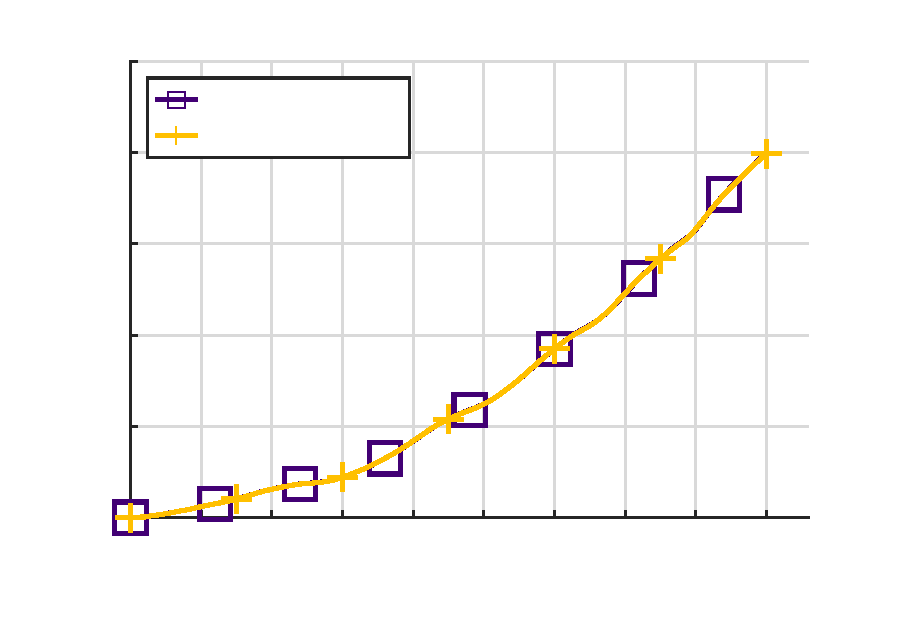
\includegraphics[scale=1]{valPropFlexThetaXO-inc}
\end{picture}%
\begin{picture}(420,288)(0,0)
\fontsize{14}{0}\selectfont\put(54.6235,36.8757){\makebox(0,0)[t]{\textcolor[rgb]{0.15,0.15,0.15}{{0}}}}
\fontsize{14}{0}\selectfont\put(88.5444,36.8757){\makebox(0,0)[t]{\textcolor[rgb]{0.15,0.15,0.15}{{50}}}}
\fontsize{14}{0}\selectfont\put(122.465,36.8757){\makebox(0,0)[t]{\textcolor[rgb]{0.15,0.15,0.15}{{100}}}}
\fontsize{14}{0}\selectfont\put(156.386,36.8757){\makebox(0,0)[t]{\textcolor[rgb]{0.15,0.15,0.15}{{150}}}}
\fontsize{14}{0}\selectfont\put(190.307,36.8757){\makebox(0,0)[t]{\textcolor[rgb]{0.15,0.15,0.15}{{200}}}}
\fontsize{14}{0}\selectfont\put(224.228,36.8757){\makebox(0,0)[t]{\textcolor[rgb]{0.15,0.15,0.15}{{250}}}}
\fontsize{14}{0}\selectfont\put(258.149,36.8757){\makebox(0,0)[t]{\textcolor[rgb]{0.15,0.15,0.15}{{300}}}}
\fontsize{14}{0}\selectfont\put(292.07,36.8757){\makebox(0,0)[t]{\textcolor[rgb]{0.15,0.15,0.15}{{350}}}}
\fontsize{14}{0}\selectfont\put(325.99,36.8757){\makebox(0,0)[t]{\textcolor[rgb]{0.15,0.15,0.15}{{400}}}}
\fontsize{14}{0}\selectfont\put(359.911,36.8757){\makebox(0,0)[t]{\textcolor[rgb]{0.15,0.15,0.15}{{450}}}}
\fontsize{14}{0}\selectfont\put(47.6312,47.3764){\makebox(0,0)[r]{\textcolor[rgb]{0.15,0.15,0.15}{{0}}}}
\fontsize{14}{0}\selectfont\put(47.6312,91.1792){\makebox(0,0)[r]{\textcolor[rgb]{0.15,0.15,0.15}{{$\pi$}}}}
\fontsize{14}{0}\selectfont\put(47.6312,134.982){\makebox(0,0)[r]{\textcolor[rgb]{0.15,0.15,0.15}{{$2\pi$}}}}
\fontsize{14}{0}\selectfont\put(47.6312,178.785){\makebox(0,0)[r]{\textcolor[rgb]{0.15,0.15,0.15}{{$3\pi$}}}}
\fontsize{14}{0}\selectfont\put(47.6312,222.588){\makebox(0,0)[r]{\textcolor[rgb]{0.15,0.15,0.15}{{$4\pi$}}}}
\fontsize{14}{0}\selectfont\put(47.6312,266.391){\makebox(0,0)[r]{\textcolor[rgb]{0.15,0.15,0.15}{{$5\pi$}}}}
\fontsize{20}{0}\selectfont\put(217.444,21.8757){\makebox(0,0)[t]{\textcolor[rgb]{0.15,0.15,0.15}{{$t$ [s]}}}}
\fontsize{20}{0}\selectfont\put(27.6312,156.884){\rotatebox{90}{\makebox(0,0)[b]{\textcolor[rgb]{0.15,0.15,0.15}{{$\theta_{x}$ [rad]}}}}}
\fontsize{12}{0}\selectfont\put(90.608,247.896){\makebox(0,0)[l]{\textcolor[rgb]{0,0,0}{{F2 (5 elements)}}}}
\fontsize{12}{0}\selectfont\put(90.608,230.898){\makebox(0,0)[l]{\textcolor[rgb]{0,0,0}{{F2 (20 elements)}}}}
\end{picture}
}
		\caption{$\theta_{x,\text{O}}(t)$.}
		\label{fig:simplePropellerFlexThetaXO}
	\end{subfigure}
	\begin{subfigure}{.45\textwidth}
		\centering
		\resizebox{\textwidth}{!}{% Title: Figure 2
% Creator: GL2PS 1.4.2, (C) 1999-2020 C. Geuzaine
% For: Octave
% CreationDate: Tue Jan 24 13:40:20 2023
\setlength{\unitlength}{1pt}
\begin{picture}(0,0)
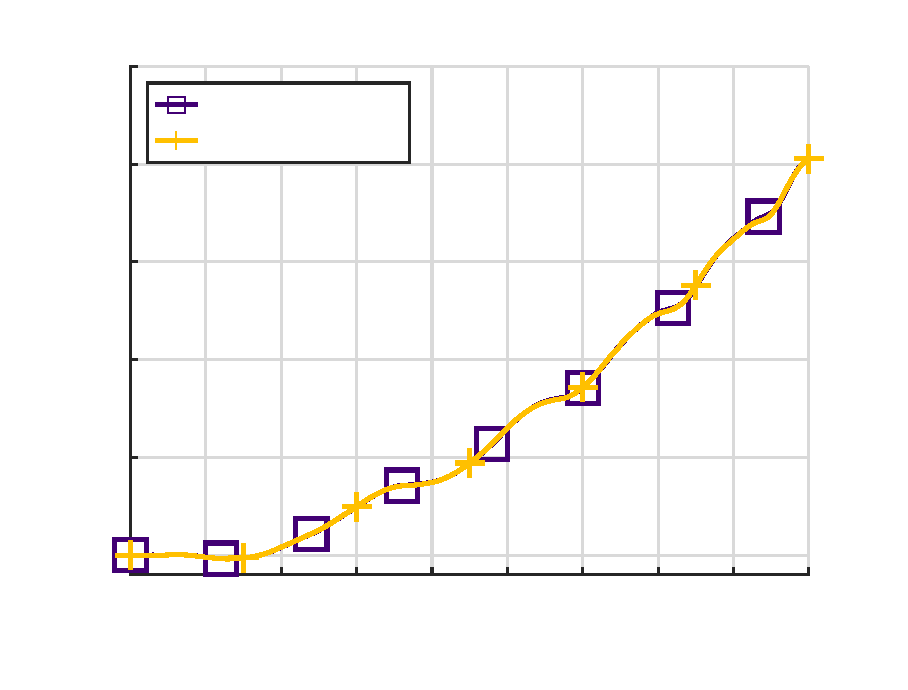
\includegraphics[scale=1]{valPropFlexThetaXA-inc}
\end{picture}%
\begin{picture}(420,315)(0,0)
\fontsize{14}{0}\selectfont\put(54.6235,36.8641){\makebox(0,0)[t]{\textcolor[rgb]{0.15,0.15,0.15}{{0}}}}
\fontsize{14}{0}\selectfont\put(90.8058,36.8641){\makebox(0,0)[t]{\textcolor[rgb]{0.15,0.15,0.15}{{50}}}}
\fontsize{14}{0}\selectfont\put(126.988,36.8641){\makebox(0,0)[t]{\textcolor[rgb]{0.15,0.15,0.15}{{100}}}}
\fontsize{14}{0}\selectfont\put(163.17,36.8641){\makebox(0,0)[t]{\textcolor[rgb]{0.15,0.15,0.15}{{150}}}}
\fontsize{14}{0}\selectfont\put(199.352,36.8641){\makebox(0,0)[t]{\textcolor[rgb]{0.15,0.15,0.15}{{200}}}}
\fontsize{14}{0}\selectfont\put(235.535,36.8641){\makebox(0,0)[t]{\textcolor[rgb]{0.15,0.15,0.15}{{250}}}}
\fontsize{14}{0}\selectfont\put(271.717,36.8641){\makebox(0,0)[t]{\textcolor[rgb]{0.15,0.15,0.15}{{300}}}}
\fontsize{14}{0}\selectfont\put(307.899,36.8641){\makebox(0,0)[t]{\textcolor[rgb]{0.15,0.15,0.15}{{350}}}}
\fontsize{14}{0}\selectfont\put(344.081,36.8641){\makebox(0,0)[t]{\textcolor[rgb]{0.15,0.15,0.15}{{400}}}}
\fontsize{14}{0}\selectfont\put(380.264,36.8641){\makebox(0,0)[t]{\textcolor[rgb]{0.15,0.15,0.15}{{450}}}}
\fontsize{14}{0}\selectfont\put(47.6312,56.7488){\makebox(0,0)[r]{\textcolor[rgb]{0.15,0.15,0.15}{{0}}}}
\fontsize{14}{0}\selectfont\put(47.6312,103.672){\makebox(0,0)[r]{\textcolor[rgb]{0.15,0.15,0.15}{{$\pi$}}}}
\fontsize{14}{0}\selectfont\put(47.6312,150.595){\makebox(0,0)[r]{\textcolor[rgb]{0.15,0.15,0.15}{{$2\pi$}}}}
\fontsize{14}{0}\selectfont\put(47.6312,197.518){\makebox(0,0)[r]{\textcolor[rgb]{0.15,0.15,0.15}{{$3\pi$}}}}
\fontsize{14}{0}\selectfont\put(47.6312,244.442){\makebox(0,0)[r]{\textcolor[rgb]{0.15,0.15,0.15}{{$4\pi$}}}}
\fontsize{14}{0}\selectfont\put(47.6312,291.365){\makebox(0,0)[r]{\textcolor[rgb]{0.15,0.15,0.15}{{$5\pi$}}}}
\fontsize{20}{0}\selectfont\put(217.444,21.8641){\makebox(0,0)[t]{\textcolor[rgb]{0.15,0.15,0.15}{{$t$ [s]}}}}
\fontsize{20}{0}\selectfont\put(27.6312,169.365){\rotatebox{90}{\makebox(0,0)[b]{\textcolor[rgb]{0.15,0.15,0.15}{{$\theta_{x,\text{A}}$ [rad]}}}}}
\fontsize{12}{0}\selectfont\put(90.608,272.87){\makebox(0,0)[l]{\textcolor[rgb]{0,0,0}{{F2 (5 elements)}}}}
\fontsize{12}{0}\selectfont\put(90.608,255.872){\makebox(0,0)[l]{\textcolor[rgb]{0,0,0}{{F2 (20 elements)}}}}
\end{picture}
}
		\caption{$\theta_{x,\text{A}}(t)$.}
		\label{fig:simplePropellerFlexThetaXA}
	\end{subfigure}
	\caption{Example 2: Flexible case results of $\theta_{x,\text{A}}(t)$ and $\theta_{x,\text{O}}(t)$ rotations.}
	\label{fig:simplePropellerFlexThetas}
\end{figure}

\clearpage 

\subsection{Example 3}

\newcommand{\CantileverBladeL}{10}
\newcommand{\CantileverBladedch}{1}
\newcommand{\CantileverBladeEeq}{14}
\newcommand{\CantileverBladeGeq}{  5.6}
\newcommand{\CantileverBladerho}{1850}
\newcommand{\CantileverBladevm}{30}
\newcommand{\CantileverBladetolF}{5}
\newcommand{\CantileverBladetolU}{1}
\newcommand{\CantileverBladedeltaT}{1}
\newcommand{\CantileverBladefinalTime}{30}
\newcommand{\CantileverBladenumElem}{10}
\newcommand{\CantileverBladealphaEnd}{   40}
\newcommand{\CantileverBladetorsionalMomentRatio}{-67745}
\newcommand{\CantileverBladetorsionalMomentFOne}{ 0.03}
\newcommand{\CantileverBladetorsionalMomentFTwo}{-1819}


\subsubsection{Parameters}
The parameters of this example are:

\begin{itemize}
	\item $d_c= \CantileverBladedch$ 
	\item $L = \CantileverBladeL$
	\item $E_{eq} = \CantileverBladeEeq$ GPa
	\item $G_{eq} = \CantileverBladeGeq$ GPa
	\item $v_{m} = \CantileverBladevm$ m/s
	\item $tol_r = \CantileverBladetolF\times 10^{-7}$
	\item $tol_u = \CantileverBladetolU0^{-15}$.
	\item $\alpha_{max} = \CantileverBladealphaEnd^{\circ}$
	
\end{itemize}


\subsubsection{Example 3: Numerical results}


The torsional moment provided by geometric nonlinearities in F1 is $\CantileverBladetorsionalMomentFOne$ N.m while using F2 is $\CantileverBladetorsionalMomentFTwo$ N.m


\begin{itemize}
	\item $d_c= \CantileverBladedch$ 
	\item $L = \CantileverBladeL$
	\item $E_{eq} = \CantileverBladeEeq$ GPa
	\item $G_{eq} = \CantileverBladeGeq$ GPa
	\item $v_{m} = \CantileverBladevm$ m/s
	\item $tol_r = \CantileverBladetolF\times 10^{-7}$
	\item $tol_u = \CantileverBladetolU0^{-15}$.
	\item $\alpha_{max} = \CantileverBladealphaEnd^{\circ}$
	
\end{itemize}


\begin{figure}[htb]
	\begin{subfigure}{.5\textwidth}
		\centering
		\resizebox{.9\textwidth}{!}{% Title: Figure 5
% Creator: GL2PS 1.4.2, (C) 1999-2020 C. Geuzaine
% For: Octave
% CreationDate: Tue Jan 24 14:16:08 2023
\setlength{\unitlength}{1pt}
\begin{picture}(0,0)
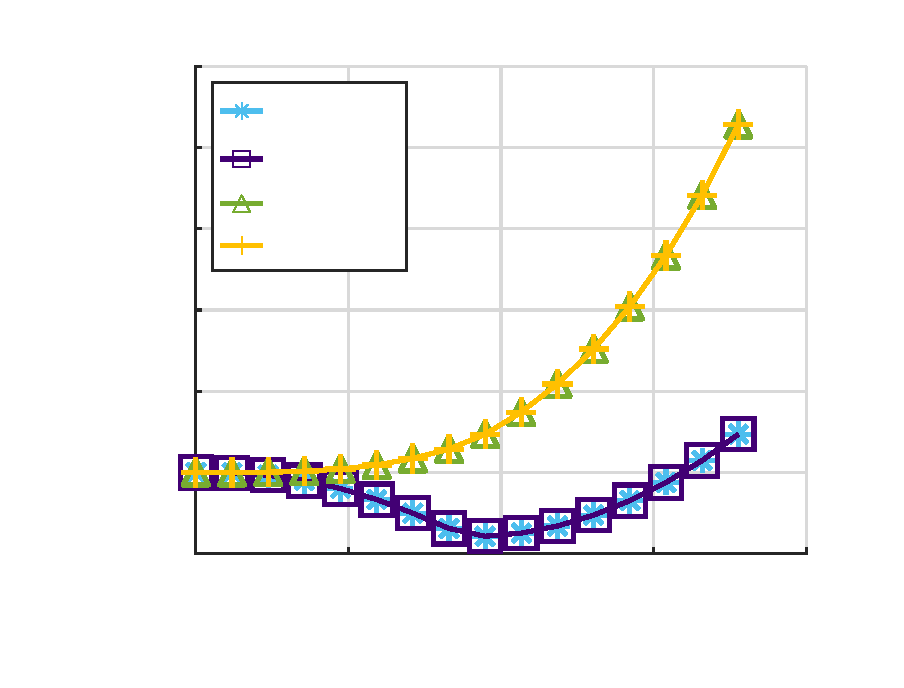
\includegraphics[scale=1]{BladeCantMomentsYZStatic-inc}
\end{picture}%
\begin{picture}(418,314)(0,0)
\fontsize{14}{0}\selectfont\put(68.999,34.9558){\makebox(0,0)[t]{\textcolor[rgb]{0.15,0.15,0.15}{{$0$}}}}
\fontsize{14}{0}\selectfont\put(146.486,34.9558){\makebox(0,0)[t]{\textcolor[rgb]{0.15,0.15,0.15}{{$\pi/16$}}}}
\fontsize{14}{0}\selectfont\put(223.973,34.9558){\makebox(0,0)[t]{\textcolor[rgb]{0.15,0.15,0.15}{{$\pi/8$}}}}
\fontsize{14}{0}\selectfont\put(301.46,34.9558){\makebox(0,0)[t]{\textcolor[rgb]{0.15,0.15,0.15}{{$3\pi/16$}}}}
\fontsize{14}{0}\selectfont\put(378.946,34.9558){\makebox(0,0)[t]{\textcolor[rgb]{0.15,0.15,0.15}{{$\pi/4$}}}}
\fontsize{14}{0}\selectfont\put(62.0002,45.4554){\makebox(0,0)[r]{\textcolor[rgb]{0.15,0.15,0.15}{{-40000}}}}
\fontsize{14}{0}\selectfont\put(62.0002,94.4537){\makebox(0,0)[r]{\textcolor[rgb]{0.15,0.15,0.15}{{-20000}}}}
\fontsize{14}{0}\selectfont\put(62.0002,143.452){\makebox(0,0)[r]{\textcolor[rgb]{0.15,0.15,0.15}{{0}}}}
\fontsize{14}{0}\selectfont\put(62.0002,192.45){\makebox(0,0)[r]{\textcolor[rgb]{0.15,0.15,0.15}{{20000}}}}
\fontsize{14}{0}\selectfont\put(62.0002,241.448){\makebox(0,0)[r]{\textcolor[rgb]{0.15,0.15,0.15}{{40000}}}}
\fontsize{14}{0}\selectfont\put(62.0002,290.447){\makebox(0,0)[r]{\textcolor[rgb]{0.15,0.15,0.15}{{60000}}}}
\fontsize{14}{0}\selectfont\put(223.973,14.9558){\makebox(0,0)[t]{\textcolor[rgb]{0.15,0.15,0.15}{{$\alpha$ [rad]}}}}
\fontsize{14}{0}\selectfont\put(17.0002,167.951){\rotatebox{90}{\makebox(0,0)[b]{\textcolor[rgb]{0.15,0.15,0.15}{{$M_z$, $M_y$ node O [N.m]}}}}}
\fontsize{12}{0}\selectfont\put(104.983,270.952){\makebox(0,0)[l]{\textcolor[rgb]{0,0,0}{{F1 $M_y$}}}}
\fontsize{12}{0}\selectfont\put(104.983,251.954){\makebox(0,0)[l]{\textcolor[rgb]{0,0,0}{{F2 $M_y$}}}}
\fontsize{12}{0}\selectfont\put(104.983,233.955){\makebox(0,0)[l]{\textcolor[rgb]{0,0,0}{{F1 $M_z$}}}}
\fontsize{12}{0}\selectfont\put(104.983,216.957){\makebox(0,0)[l]{\textcolor[rgb]{0,0,0}{{F2 $M_z$}}}}
\end{picture}
}		
		\caption{$M_y, M_z(\alpha)$.}
		\label{fig:BladeCantMYMZStatic}
	\end{subfigure}
	\begin{subfigure}{0.5\textwidth}
		\centering
		\resizebox{.9\textwidth}{!}{% Title: Figure 3
% Creator: GL2PS 1.4.2, (C) 1999-2020 C. Geuzaine
% For: Octave
% CreationDate: Sat Jan 21 18:26:39 2023
\setlength{\unitlength}{1pt}
\begin{picture}(0,0)
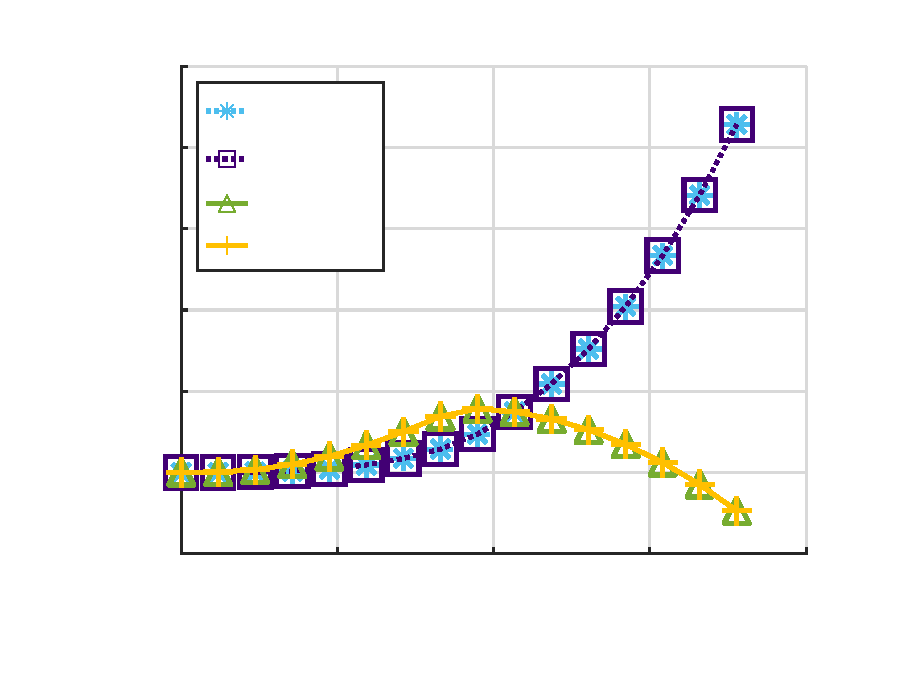
\includegraphics[scale=1]{BladeCantForcesStatic-inc}
\end{picture}%
\begin{picture}(418,314)(0,0)
\fontsize{18}{0}\selectfont\put(78.998,42.9569){\makebox(0,0)[t]{\textcolor[rgb]{0.15,0.15,0.15}{{$0$}}}}
\fontsize{18}{0}\selectfont\put(153.985,42.9569){\makebox(0,0)[t]{\textcolor[rgb]{0.15,0.15,0.15}{{$\pi/16$}}}}
\fontsize{18}{0}\selectfont\put(228.972,42.9569){\makebox(0,0)[t]{\textcolor[rgb]{0.15,0.15,0.15}{{$\pi/8$}}}}
\fontsize{18}{0}\selectfont\put(303.959,42.9569){\makebox(0,0)[t]{\textcolor[rgb]{0.15,0.15,0.15}{{$3\pi/16$}}}}
\fontsize{18}{0}\selectfont\put(378.946,42.9569){\makebox(0,0)[t]{\textcolor[rgb]{0.15,0.15,0.15}{{$\pi/4$}}}}
\fontsize{18}{0}\selectfont\put(69.9996,56.4563){\makebox(0,0)[r]{\textcolor[rgb]{0.15,0.15,0.15}{{-2000}}}}
\fontsize{18}{0}\selectfont\put(69.9996,95.4547){\makebox(0,0)[r]{\textcolor[rgb]{0.15,0.15,0.15}{{0}}}}
\fontsize{18}{0}\selectfont\put(69.9996,134.453){\makebox(0,0)[r]{\textcolor[rgb]{0.15,0.15,0.15}{{2000}}}}
\fontsize{18}{0}\selectfont\put(69.9996,173.452){\makebox(0,0)[r]{\textcolor[rgb]{0.15,0.15,0.15}{{4000}}}}
\fontsize{18}{0}\selectfont\put(69.9996,212.45){\makebox(0,0)[r]{\textcolor[rgb]{0.15,0.15,0.15}{{6000}}}}
\fontsize{18}{0}\selectfont\put(69.9996,251.448){\makebox(0,0)[r]{\textcolor[rgb]{0.15,0.15,0.15}{{8000}}}}
\fontsize{18}{0}\selectfont\put(69.9996,290.447){\makebox(0,0)[r]{\textcolor[rgb]{0.15,0.15,0.15}{{10000}}}}
\fontsize{18}{0}\selectfont\put(228.972,18.9569){\makebox(0,0)[t]{\textcolor[rgb]{0.15,0.15,0.15}{{$\alpha$ [rad]}}}}
\fontsize{18}{0}\selectfont\put(20.9996,173.452){\rotatebox{90}{\makebox(0,0)[b]{\textcolor[rgb]{0.15,0.15,0.15}{{$F_y$, $F_z$ node O [N]}}}}}
\fontsize{16}{0}\selectfont\put(114.982,268.952){\makebox(0,0)[l]{\textcolor[rgb]{0,0,0}{{F1 $F_y$}}}}
\fontsize{16}{0}\selectfont\put(114.982,245.954){\makebox(0,0)[l]{\textcolor[rgb]{0,0,0}{{F2 $F_y$}}}}
\fontsize{16}{0}\selectfont\put(114.982,224.455){\makebox(0,0)[l]{\textcolor[rgb]{0,0,0}{{F1 $F_z$}}}}
\fontsize{16}{0}\selectfont\put(114.982,204.457){\makebox(0,0)[l]{\textcolor[rgb]{0,0,0}{{F2 $F_z$}}}}
\end{picture}
}		
		\caption{$F_y$, $F_z$ $(\alpha)$.}
		\label{fig:BladeCantForcesStatic}
	\end{subfigure}
	\caption{Example 3: Reaction bending moments $M_y(\alpha)$, $M_z(\alpha)$ and resultant shear forces $F_y(\alpha)$ and $F_z(\alpha)$ at node O.}
	\label{fig:BladeCantStaticBending}
\end{figure}

\begin{figure}[htb]
	\centering
	\resizebox{.45\textwidth}{!}{% Title: Figure 4
% Creator: GL2PS 1.4.2, (C) 1999-2020 C. Geuzaine
% For: Octave
% CreationDate: Mon Jan 23 19:18:42 2023
\setlength{\unitlength}{1pt}
\begin{picture}(0,0)
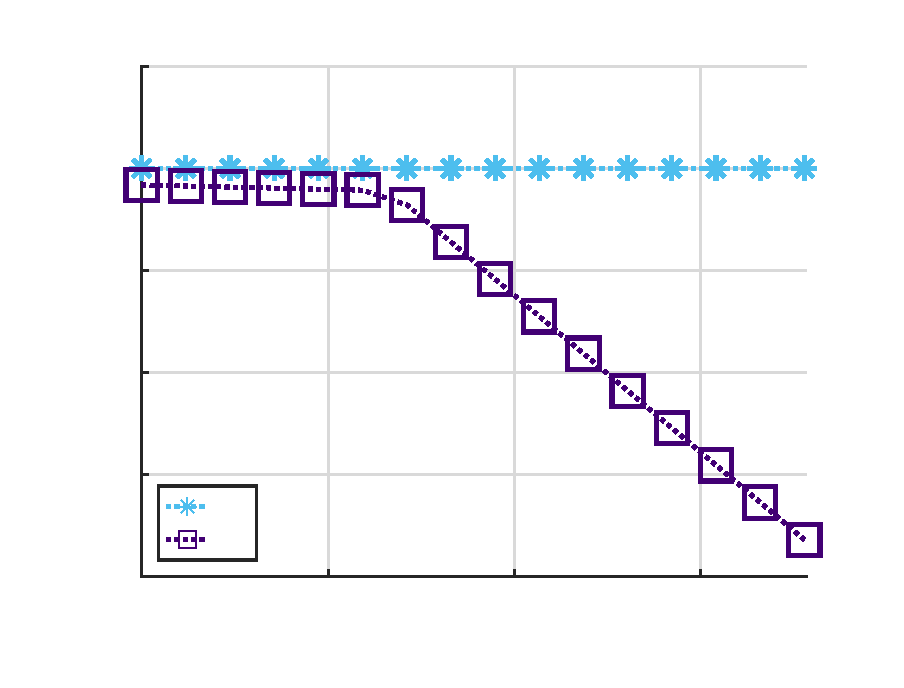
\includegraphics[scale=1]{BladeCantMomentXStatic-inc}
\end{picture}%
\begin{picture}(418,314)(0,0)
\fontsize{18}{0}\selectfont\put(74.9985,42.9569){\makebox(0,0)[t]{\textcolor[rgb]{0.15,0.15,0.15}{{$0$}}}}
\fontsize{18}{0}\selectfont\put(160.256,42.9569){\makebox(0,0)[t]{\textcolor[rgb]{0.15,0.15,0.15}{{$\pi/16$}}}}
\fontsize{18}{0}\selectfont\put(245.513,42.9569){\makebox(0,0)[t]{\textcolor[rgb]{0.15,0.15,0.15}{{$\pi/8$}}}}
\fontsize{18}{0}\selectfont\put(330.77,42.9569){\makebox(0,0)[t]{\textcolor[rgb]{0.15,0.15,0.15}{{$3\pi/16$}}}}
\fontsize{18}{0}\selectfont\put(66,56.4563){\makebox(0,0)[r]{\textcolor[rgb]{0.15,0.15,0.15}{{-2000}}}}
\fontsize{18}{0}\selectfont\put(66,103.254){\makebox(0,0)[r]{\textcolor[rgb]{0.15,0.15,0.15}{{-1500}}}}
\fontsize{18}{0}\selectfont\put(66,150.052){\makebox(0,0)[r]{\textcolor[rgb]{0.15,0.15,0.15}{{-1000}}}}
\fontsize{18}{0}\selectfont\put(66,196.851){\makebox(0,0)[r]{\textcolor[rgb]{0.15,0.15,0.15}{{-500}}}}
\fontsize{18}{0}\selectfont\put(66,243.649){\makebox(0,0)[r]{\textcolor[rgb]{0.15,0.15,0.15}{{0}}}}
\fontsize{18}{0}\selectfont\put(66,290.447){\makebox(0,0)[r]{\textcolor[rgb]{0.15,0.15,0.15}{{500}}}}
\fontsize{18}{0}\selectfont\put(226.972,18.9568){\makebox(0,0)[t]{\textcolor[rgb]{0.15,0.15,0.15}{{$\alpha$ [rad]}}}}
\fontsize{18}{0}\selectfont\put(19,173.452){\rotatebox{90}{\makebox(0,0)[b]{\textcolor[rgb]{0.15,0.15,0.15}{{$M_x$ node O [N.m]}}}}}
\fontsize{16}{0}\selectfont\put(110.983,95.1194){\makebox(0,0)[l]{\textcolor[rgb]{0,0,0}{{F1}}}}
\fontsize{16}{0}\selectfont\put(110.983,76.0077){\makebox(0,0)[l]{\textcolor[rgb]{0,0,0}{{F2}}}}
\end{picture}
}
	\caption{Example 3: Torsional moment $M_x(\alpha)$ at node O.}
	\label{fig:BladeCantMXStatic}
\end{figure}


\clearpage 

\subsection{Example 4}

\newcommand{\WindTurbineL}{10}
\newcommand{\WindTurbinedch}{1}
\newcommand{\WindTurbineEeq}{14}
\newcommand{\WindTurbineGeq}{5.6}
\newcommand{\WindTurbinerhoeq}{1850}
\newcommand{\WindTurbineva}{27}
\newcommand{\WindTurbinetolF}{1}
\newcommand{\WindTurbinetolU}{1}
\newcommand{\WindTurbinedeltaT}{0.01}
\newcommand{\WindTurbinefinalTime}{30}
\newcommand{\WindTurbineelemBlade}{30}
\newcommand{\WindTurbinenumRev}{    7}


\subsubsection{Parameters}

The parameters of the blade simulated in this example are the same as used the previous example. 
\begin{itemize}
	\item $L = \WindTurbineL$ m.
	\item $d_{ch} = \WindTurbinedch$ m.
	\item $E = \WindTurbineEeq$ GPa. 
	\item $G = \WindTurbineGeq$ GPa. 
	\item $t_f = \WindTurbinefinalTime$ s.
	\item $\Delta_t = \WindTurbinedeltaT$ s.
	\item  $tol_r = \WindTurbinetolF0^{-5}$.
	\item $tol_u = \WindTurbinetolU0^{-10}$.
	\item $\WindTurbineelemBlade$ elements per blade.
\end{itemize}



\begin{figure}[htb]
	\begin{subfigure}{0.5\textwidth}
		\centering
		\resizebox{\textwidth}{!}{% Title: Figure 1
% Creator: GL2PS 1.4.2, (C) 1999-2020 C. Geuzaine
% For: Octave
% CreationDate: Mon Jan 23 22:17:24 2023
\setlength{\unitlength}{1pt}
\begin{picture}(0,0)
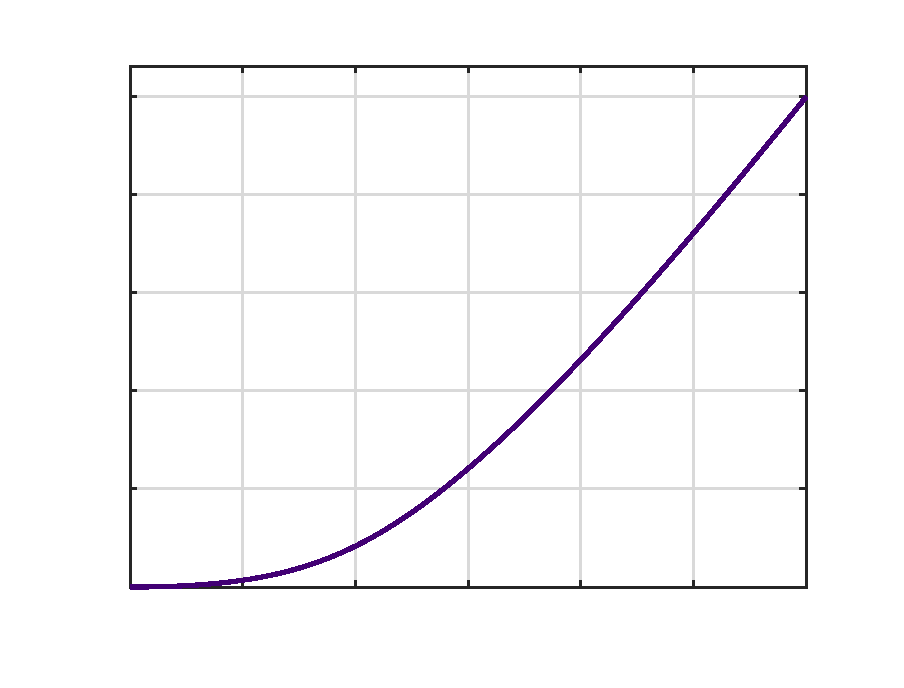
\includegraphics[scale=1]{thetaX-inc}
\end{picture}%
\begin{picture}(418,314)(0,0)
\fontsize{14}{0}\selectfont\put(54.4343,29.9561){\makebox(0,0)[t]{\textcolor[rgb]{0.15,0.15,0.15}{{0}}}}
\fontsize{14}{0}\selectfont\put(108.52,29.9561){\makebox(0,0)[t]{\textcolor[rgb]{0.15,0.15,0.15}{{5}}}}
\fontsize{14}{0}\selectfont\put(162.605,29.9561){\makebox(0,0)[t]{\textcolor[rgb]{0.15,0.15,0.15}{{10}}}}
\fontsize{14}{0}\selectfont\put(216.69,29.9561){\makebox(0,0)[t]{\textcolor[rgb]{0.15,0.15,0.15}{{15}}}}
\fontsize{14}{0}\selectfont\put(270.776,29.9561){\makebox(0,0)[t]{\textcolor[rgb]{0.15,0.15,0.15}{{20}}}}
\fontsize{14}{0}\selectfont\put(324.861,29.9561){\makebox(0,0)[t]{\textcolor[rgb]{0.15,0.15,0.15}{{25}}}}
\fontsize{14}{0}\selectfont\put(378.946,29.9561){\makebox(0,0)[t]{\textcolor[rgb]{0.15,0.15,0.15}{{30}}}}
\fontsize{14}{0}\selectfont\put(47.4448,40.4557){\makebox(0,0)[r]{\textcolor[rgb]{0.15,0.15,0.15}{{0}}}}
\fontsize{14}{0}\selectfont\put(47.4448,87.5779){\makebox(0,0)[r]{\textcolor[rgb]{0.15,0.15,0.15}{{$3\pi$}}}}
\fontsize{14}{0}\selectfont\put(47.4448,134.7){\makebox(0,0)[r]{\textcolor[rgb]{0.15,0.15,0.15}{{$6\pi$}}}}
\fontsize{14}{0}\selectfont\put(47.4448,181.822){\makebox(0,0)[r]{\textcolor[rgb]{0.15,0.15,0.15}{{$9\pi$}}}}
\fontsize{14}{0}\selectfont\put(47.4448,228.944){\makebox(0,0)[r]{\textcolor[rgb]{0.15,0.15,0.15}{{$12\pi$}}}}
\fontsize{14}{0}\selectfont\put(47.4448,276.067){\makebox(0,0)[r]{\textcolor[rgb]{0.15,0.15,0.15}{{$15\pi$}}}}
\fontsize{14}{0}\selectfont\put(216.69,14.9561){\makebox(0,0)[t]{\textcolor[rgb]{0.15,0.15,0.15}{{$t$ [s]}}}}
\fontsize{14}{0}\selectfont\put(21.4448,165.451){\rotatebox{90}{\makebox(0,0)[b]{\textcolor[rgb]{0.15,0.15,0.15}{{$\theta_x$ node O [rad]}}}}}
\end{picture}
}
		\caption{$\theta_x(t)$ node O.}
		\label{fig:windTurbineThetaXO}
	\end{subfigure}
	\begin{subfigure}{.5\textwidth}
		\centering
		\resizebox{\textwidth}{!}{% Title: Figure 2
% Creator: GL2PS 1.4.2, (C) 1999-2020 C. Geuzaine
% For: Octave
% CreationDate: Mon Jan 23 22:17:24 2023
\setlength{\unitlength}{1pt}
\begin{picture}(0,0)
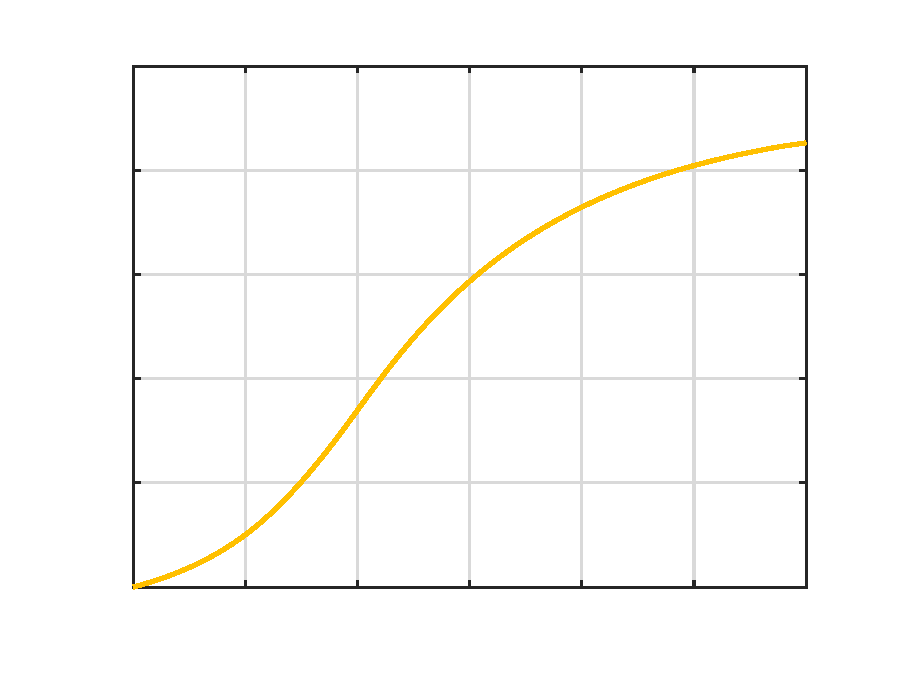
\includegraphics[scale=1]{thetadotX-inc}
\end{picture}%
\begin{picture}(418,314)(0,0)
\fontsize{14}{0}\selectfont\put(55.999,29.9561){\makebox(0,0)[t]{\textcolor[rgb]{0.15,0.15,0.15}{{0}}}}
\fontsize{14}{0}\selectfont\put(109.824,29.9561){\makebox(0,0)[t]{\textcolor[rgb]{0.15,0.15,0.15}{{5}}}}
\fontsize{14}{0}\selectfont\put(163.648,29.9561){\makebox(0,0)[t]{\textcolor[rgb]{0.15,0.15,0.15}{{10}}}}
\fontsize{14}{0}\selectfont\put(217.473,29.9561){\makebox(0,0)[t]{\textcolor[rgb]{0.15,0.15,0.15}{{15}}}}
\fontsize{14}{0}\selectfont\put(271.297,29.9561){\makebox(0,0)[t]{\textcolor[rgb]{0.15,0.15,0.15}{{20}}}}
\fontsize{14}{0}\selectfont\put(325.122,29.9561){\makebox(0,0)[t]{\textcolor[rgb]{0.15,0.15,0.15}{{25}}}}
\fontsize{14}{0}\selectfont\put(378.946,29.9561){\makebox(0,0)[t]{\textcolor[rgb]{0.15,0.15,0.15}{{30}}}}
\fontsize{14}{0}\selectfont\put(49.0002,40.4557){\makebox(0,0)[r]{\textcolor[rgb]{0.15,0.15,0.15}{{0}}}}
\fontsize{14}{0}\selectfont\put(49.0002,90.4539){\makebox(0,0)[r]{\textcolor[rgb]{0.15,0.15,0.15}{{$\pi/5$}}}}
\fontsize{14}{0}\selectfont\put(49.0002,140.452){\makebox(0,0)[r]{\textcolor[rgb]{0.15,0.15,0.15}{{$2\pi/5$}}}}
\fontsize{14}{0}\selectfont\put(49.0002,190.45){\makebox(0,0)[r]{\textcolor[rgb]{0.15,0.15,0.15}{{$3\pi/5$}}}}
\fontsize{14}{0}\selectfont\put(49.0002,240.449){\makebox(0,0)[r]{\textcolor[rgb]{0.15,0.15,0.15}{{$4\pi/5$}}}}
\fontsize{14}{0}\selectfont\put(49.0002,290.447){\makebox(0,0)[r]{\textcolor[rgb]{0.15,0.15,0.15}{{$\pi$}}}}
\fontsize{14}{0}\selectfont\put(217.473,14.9561){\makebox(0,0)[t]{\textcolor[rgb]{0.15,0.15,0.15}{{$t$ [s]}}}}
\fontsize{14}{0}\selectfont\put(15.0002,165.451){\rotatebox{90}{\makebox(0,0)[b]{\textcolor[rgb]{0.15,0.15,0.15}{{$\dot{\theta_x}$ node O [rad/s]}}}}}
\end{picture}
}
		\caption{$\dot{\theta_x}(t)$ node O.}
		\label{fig:windTurbineThetadotXO}
	\end{subfigure}
	\caption{Example 4: $\theta_x$ angle and velocity rotation.}
	\label{fig:windTurbineThetaX0}
\end{figure}


\begin{figure}[htb]                  
	\centering                         
	\resizebox{.5\textwidth}{!}{% Title: Figure 3
% Creator: GL2PS 1.4.2, (C) 1999-2020 C. Geuzaine
% For: Octave
% CreationDate: Mon Jan 23 22:17:25 2023
\setlength{\unitlength}{1pt}
\begin{picture}(0,0)
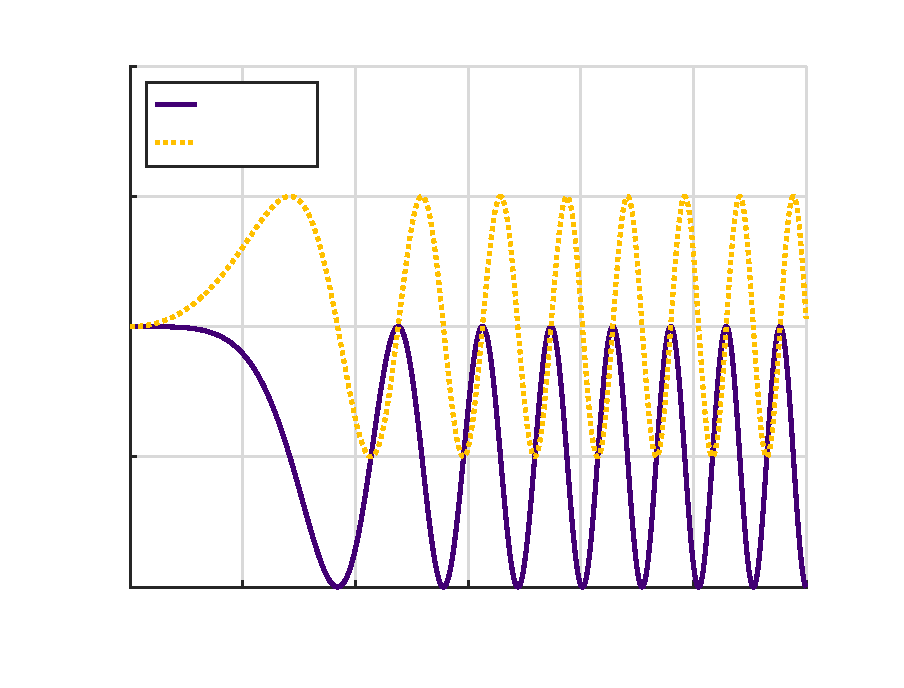
\includegraphics[scale=1]{dispsA-inc}
\end{picture}%
\begin{picture}(418,314)(0,0)
\fontsize{14}{0}\selectfont\put(54.4343,29.9561){\makebox(0,0)[t]{\textcolor[rgb]{0.15,0.15,0.15}{{0}}}}
\fontsize{14}{0}\selectfont\put(108.52,29.9561){\makebox(0,0)[t]{\textcolor[rgb]{0.15,0.15,0.15}{{5}}}}
\fontsize{14}{0}\selectfont\put(162.605,29.9561){\makebox(0,0)[t]{\textcolor[rgb]{0.15,0.15,0.15}{{10}}}}
\fontsize{14}{0}\selectfont\put(216.69,29.9561){\makebox(0,0)[t]{\textcolor[rgb]{0.15,0.15,0.15}{{15}}}}
\fontsize{14}{0}\selectfont\put(270.776,29.9561){\makebox(0,0)[t]{\textcolor[rgb]{0.15,0.15,0.15}{{20}}}}
\fontsize{14}{0}\selectfont\put(324.861,29.9561){\makebox(0,0)[t]{\textcolor[rgb]{0.15,0.15,0.15}{{25}}}}
\fontsize{14}{0}\selectfont\put(378.946,29.9561){\makebox(0,0)[t]{\textcolor[rgb]{0.15,0.15,0.15}{{30}}}}
\fontsize{14}{0}\selectfont\put(47.4448,40.4557){\makebox(0,0)[r]{\textcolor[rgb]{0.15,0.15,0.15}{{-20}}}}
\fontsize{14}{0}\selectfont\put(47.4448,102.953){\makebox(0,0)[r]{\textcolor[rgb]{0.15,0.15,0.15}{{-10}}}}
\fontsize{14}{0}\selectfont\put(47.4448,165.451){\makebox(0,0)[r]{\textcolor[rgb]{0.15,0.15,0.15}{{0}}}}
\fontsize{14}{0}\selectfont\put(47.4448,227.949){\makebox(0,0)[r]{\textcolor[rgb]{0.15,0.15,0.15}{{10}}}}
\fontsize{14}{0}\selectfont\put(47.4448,290.447){\makebox(0,0)[r]{\textcolor[rgb]{0.15,0.15,0.15}{{20}}}}
\fontsize{14}{0}\selectfont\put(216.69,14.9561){\makebox(0,0)[t]{\textcolor[rgb]{0.15,0.15,0.15}{{$t$ [s]}}}}
\fontsize{14}{0}\selectfont\put(23.4448,165.451){\rotatebox{90}{\makebox(0,0)[b]{\textcolor[rgb]{0.15,0.15,0.15}{{ $u_z$, $u_y$ (A) [m]}}}}}
\fontsize{12}{0}\selectfont\put(90.4186,271.952){\makebox(0,0)[l]{\textcolor[rgb]{0,0,0}{{\text{$u_z$}}}}}
\fontsize{12}{0}\selectfont\put(90.4186,253.954){\makebox(0,0)[l]{\textcolor[rgb]{0,0,0}{{\text{$u_y$}}}}}
\end{picture}
}
	\caption{Example 4: Displacements $u_y(t)$ and $u_z(t)$ of node A.}
	\label{fig:windTurbineDispsA}
\end{figure}




\end{document}
